%!TEX root = ../thesis.tex

\chapter{Results}
\label{chap:r}

In the previous chapter, I described the workings of my processing pipeline, giving a detailed account of the algorithms and procedures that take place in each pipeline step. These descriptions included discussion related to design decisions and modifications to the original plans. These were mostly based, in fact, on my results, or more accurately, on my experience at implementing the methods and testing how effectively they were achieving the goals set out for them. Being the result of a process of iterative refinement and revision, the final methods and results of this research are deeply interlinked and are thus difficult to separate into two chapters. The above describes one such overlap.

In this section, I will focus not on how preliminary results affected the pipeline, or how the results evolved as a function of changes to the pipeline, as I already addressed this topic in the previous chapter. Instead, I will restrict the discussion to focus only on the \textit{final} relationship between the final version of the code and the outputs it produces.

In the following sections, I will show the intermediate results of each step of the pipeline visually in figures, as well as describe them in the text. This showcase and description of the results will focus primarily on the strengths and weaknesses of each part of the implementation, creating links between the underlying methods and features in the output. These sections describe how successful the methods are based on the visual inspection of the outputs, as well as my experience in developing the implementation and working with the data.

The last part of the chapter contains a section in which the results of quantifying the quality and accuracy of the output are shown and discussed, followed by a section in which the commercial results and the present academic results are compared, especially in terms of the overall quality of the results they produce.

\subsection{Manual pre-processing}
\label{sub:manualpreprocessing}

Implementing a scaling solution did not form part of this project, although all parts of the implementation were designed in a way that a binary production version of it would have manageable computational complexity and could be embedded in a scaling framework with a relatively small amount of effort. Scaling in this project concerns primarily the need to subdivide the input data in a way that the software can queue up portions of it for parallel computation and never run out of memory while processing a set number of these portions. These portions could be generated, in the simplest case, based on tiling, i.e. overlaying a 2D raster on the extents of the data and examining which cell certain features fall into.

As scaling was not part of this project, the task of creating such manageable subsets of the input data was carried out manually prior to starting development on the main processing steps. This procedure consisted of cropping the input vector datasets into tiles showing interesting 3D features (important for testing), and for each of them, retaining only those Lidar points which fall within their extents \textit{and} are a set maximum distance from any roads in their respective NWB tiles. For the former task, I used the vector operations toolset in QGIS, and for the latter I used LASTools.

I derived the area of interest in which to keep Lidar points by buffering the centrelines in NWB tiles by 150 metres, and passing these geometries on to LASTools to use to \textit{clip} AHN3 tiles. AHN3 itself comes tiled in the official release (on a much larger scale), and I derived each testing dataset from a single AHN3 tile to keep the manual procedure simple. I also discarded AHN3 points not classed as ground or bridge points (2 and 26 respectively), since these are the only points in AHN3 that could be relevant to the task of characterising road surfaces. This is explained in more depth in Section [REF]. 

Visualisations are shown in Figure \ref{fig:manualpreprocessing} in which an NWB "tile" and the Lidar clipping polygon (on the left) is shown alongside the clipped Lidar tile (on the right). The clipping polygon was manually edited to have sharp, linear boundaries and NWB wegvakken (yellow lines) touching its interior (red areas) were included in the testing dataset. This also allowed me to test how well the procedure performs in areas where AHN3 is completely unavailable for a short distance, but where DTB coverage is present (not shown in this figure). On the right, the point cloud is shown in its original density, not a derived DTM. Darker areas represent lower elevations, the total elevation range shown in the image is about ten metres. Ultimately, the process resulted in the 11 testing datasets, each with its own cropped NWB, DTB and AHN3 files, which are described in the next section. The dataset shown in this figure is Knoppunt Deil (from AHN3 tile 39CZ1).

I picked 150 metres as a buffer distance for the Lidar clipping not because I expected road surfaces to be so wide, but because I found that it reduced the volume of points to manageable levels in my testing tiles, while retaining plenty of neighbourhood information, which I found to be useful for debugging purposes, and for the assessment of how well my algorithms perform in various environments next to roads. Using a smaller buffer distance would lead to slightly reduced runtimes, but by a very small margin. Input point cloud thinning, on the other hand, is a major control on both runtimes and output accuracy, which will be discussed in the context of the most affected pipeline steps below.

\subsection{Testing datasets}
\label{sub:testingdata}

The secondary goal in producing the testing datasets was to make their size manageable (especially with regards to the clipped point clouds), so that debugging times can be kept low. At the same time, I kept in mind that the set of chosen areas needed to be representative of the whole country to provide an insight into the computational complexity and visual performance of the algorithm in as many scenarios as possible. Furthermore, I also deliberately included areas which I thought would prove especially problematic, such as roads with tunnels, frequent stationary vehicles and challenging, multi-level 3D relationships (in motorway interchanges). Table \ref{tab:inventory} provides an inventory of all the datasets I experimented and tested with. The tile identifier in the first column refers to those used in \cite{ahn3_download}; each dataset is found within a single AHN3 tile as I mentioned in the last section. The resulting datasets fit into memory easily even on a mediocre computer, and are also small enough to allow intermediate results to be visualised and interpreted quickly.

\begin{longtable}[c]{@{}p{2.8cm}p{6.8cm}c@{}}
\toprule
Title, tile  & Features & Render \\ \midrule
Markerwarddijk, 20BN1 & P-road on a dike in the Markermeer. Very limited amount of terrain around the road. Road consistently build on ground, there are no bridge structures. & \raisebox{-0.94\totalheight}{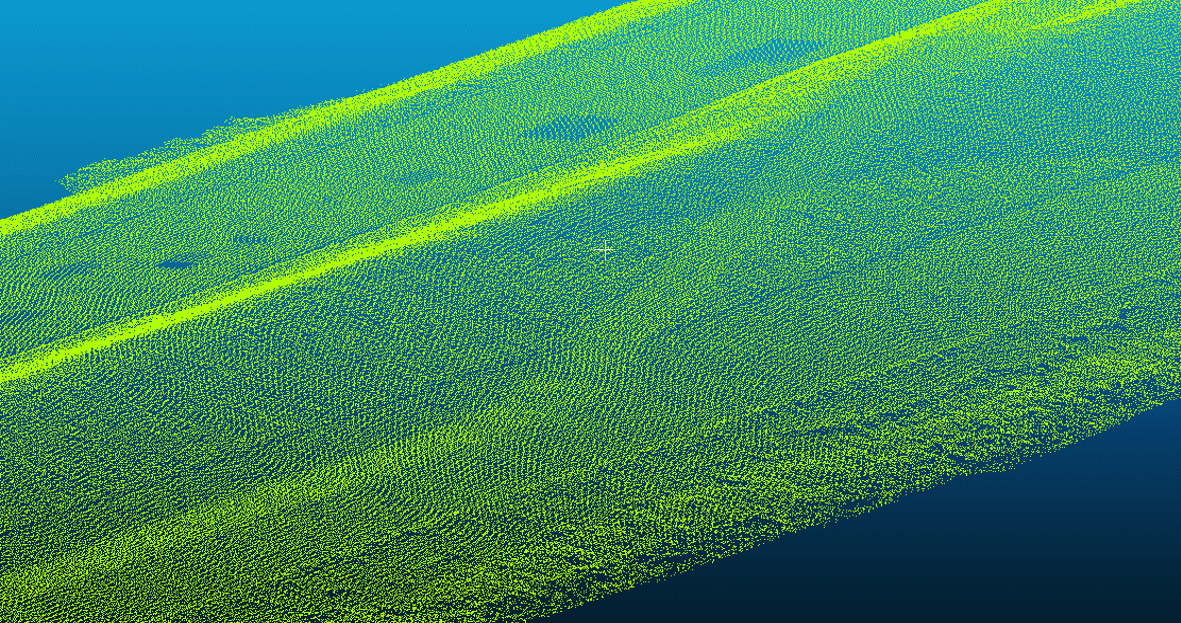
\includegraphics[width=6cm, height=3.5cm]{final_report/figs/ahn_sample_20BN1_a.png}}  \\
Amsterdam Hemhavens, 25BZ2 & Ringweg-West (R-road) as it crosses the IJ through the Coentunnel in a densely built-up environment. It is built on artificially elevated ground and on bridges in this area. Part of Westradweg also included, built entirely on a long bridge. & \raisebox{-0.94\totalheight}{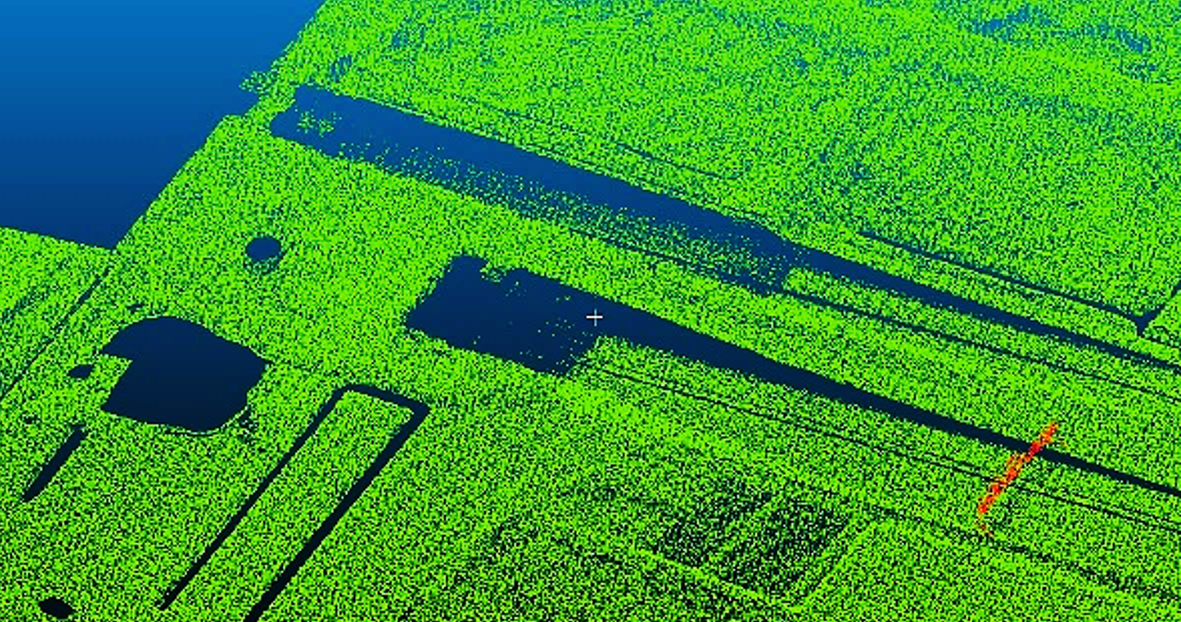
\includegraphics[width=6cm, height=3.5cm]{final_report/figs/ahn_sample_25BZ2_a.png}} \\
Amsterdam Zuid, 25DN2 & R-roads with many closely spaced bridges, small tunnels, dense grouping of holes around roads due to presence of water and buildings & \raisebox{-0.94\totalheight}{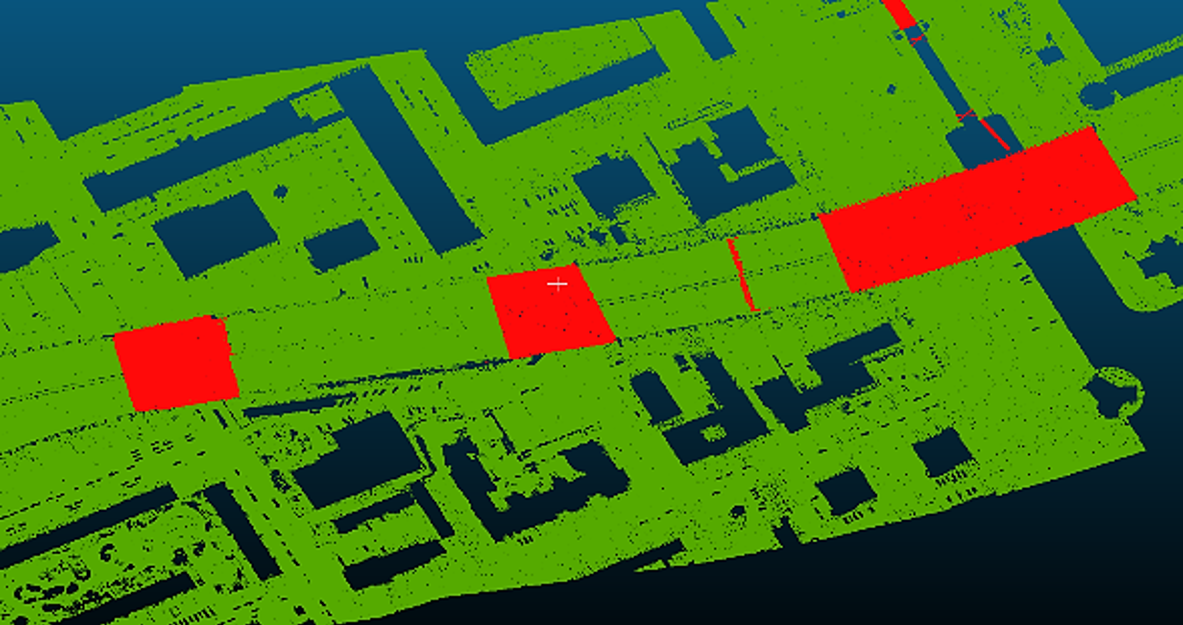
\includegraphics[width=6cm, height=3.5cm]{final_report/figs/ahn_sample_25DN2_a.png}} \\
Bunschoten, 32BN1 & P-roads with three big roundabouts, and one road that ends in a small roundabout. Amersfoortseweg has its two lanes on separate road surfaces (like motorways), but with frequent connecting segments. & \raisebox{-0.94\totalheight}{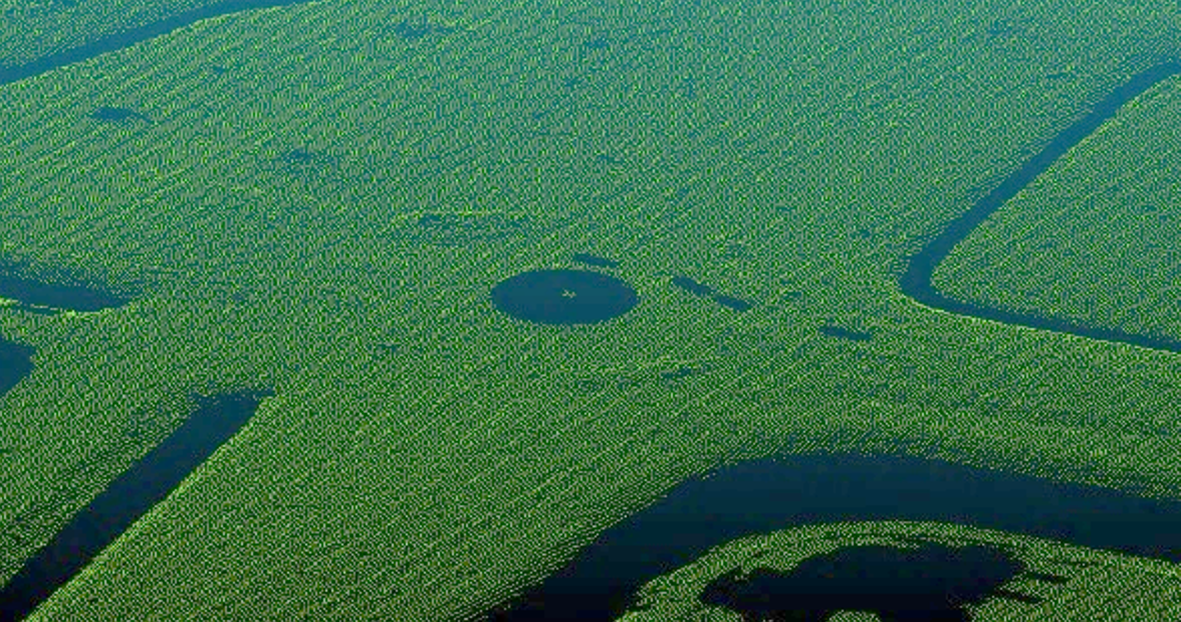
\includegraphics[width=6cm, height=3.5cm]{final_report/figs/ahn_sample_32BN1_a.png}} \\
Veluwe, 32FZ2 & Straight R-roads surrounded by dense forest and crossed by wide wildlife overpasses. & \raisebox{-0.94\totalheight}{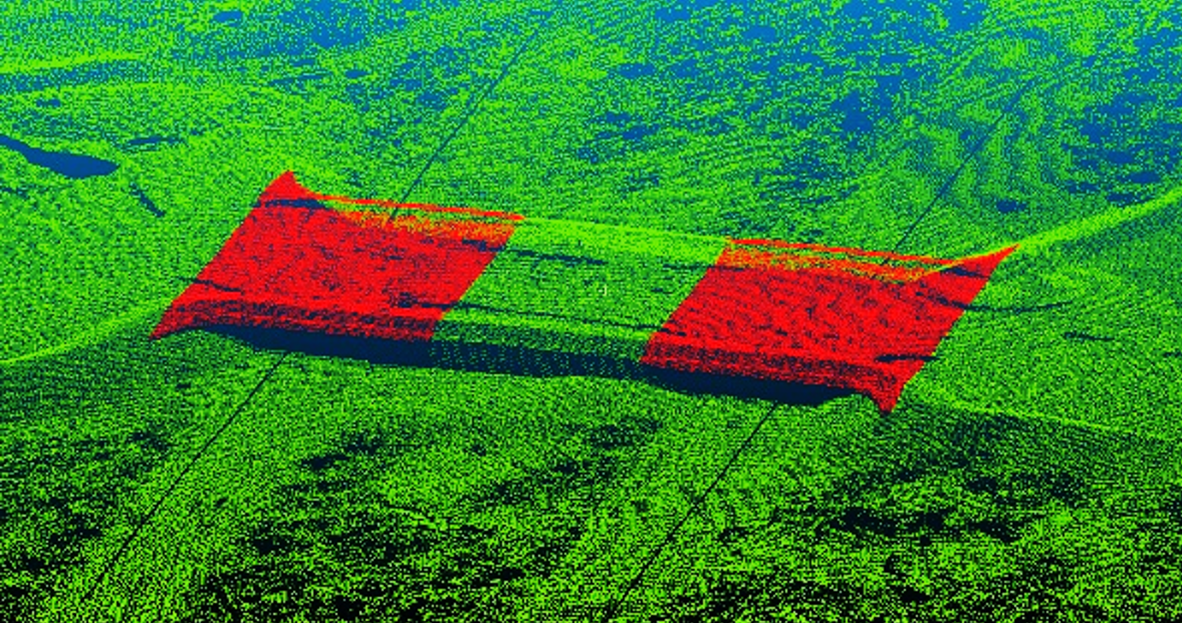
\includegraphics[width=6cm, height=3.5cm]{final_report/figs/ahn_sample_32FZ2_a.png}} \\
Apeldoornseweg, 32HZ2 & P-road in dense forest with canopy frequently occluding the road surface, decreasing point density and occasionally creating gaps. The road has small parallel branches running very close to it, which may make it difficult for the algorithm to distinguish between them. It also has roundabouts. & \raisebox{-0.94\totalheight}{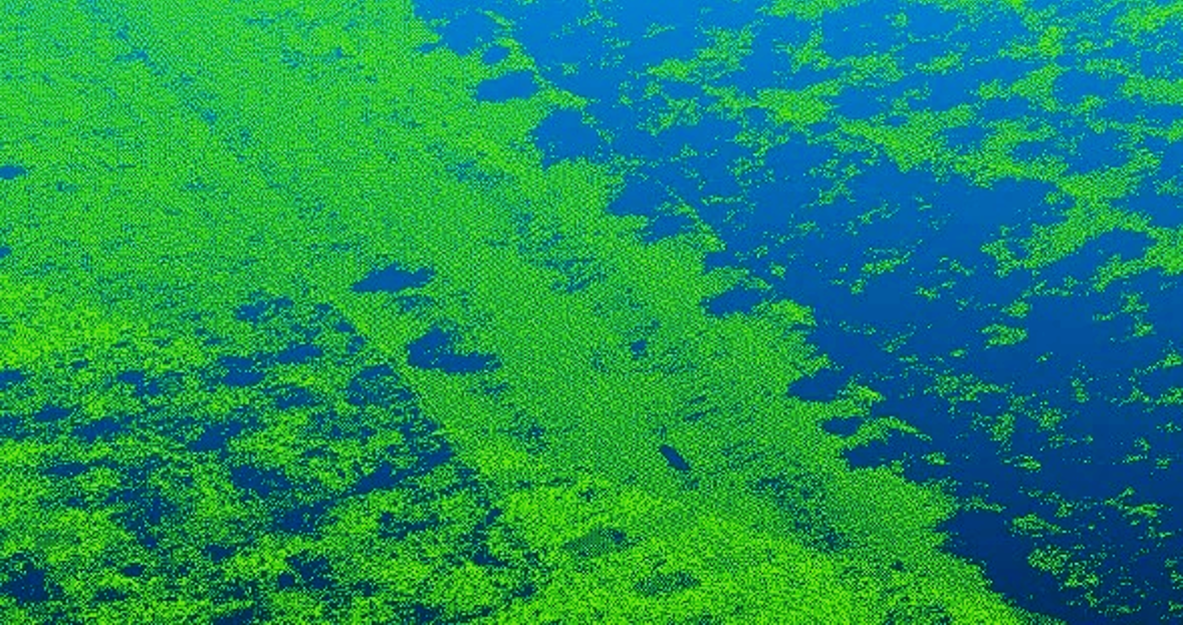
\includegraphics[width=6cm, height=3.5cm]{final_report/figs/ahn_sample_32HZ2_a.png}} \\
Hoenderloo, 33CN2 & P-road in extremely dense, continuous forest with canopy frequently occluding the road surface, decreasing point density and occasionally creating gaps. Both lanes are on the same road surface & \raisebox{-0.94\totalheight}{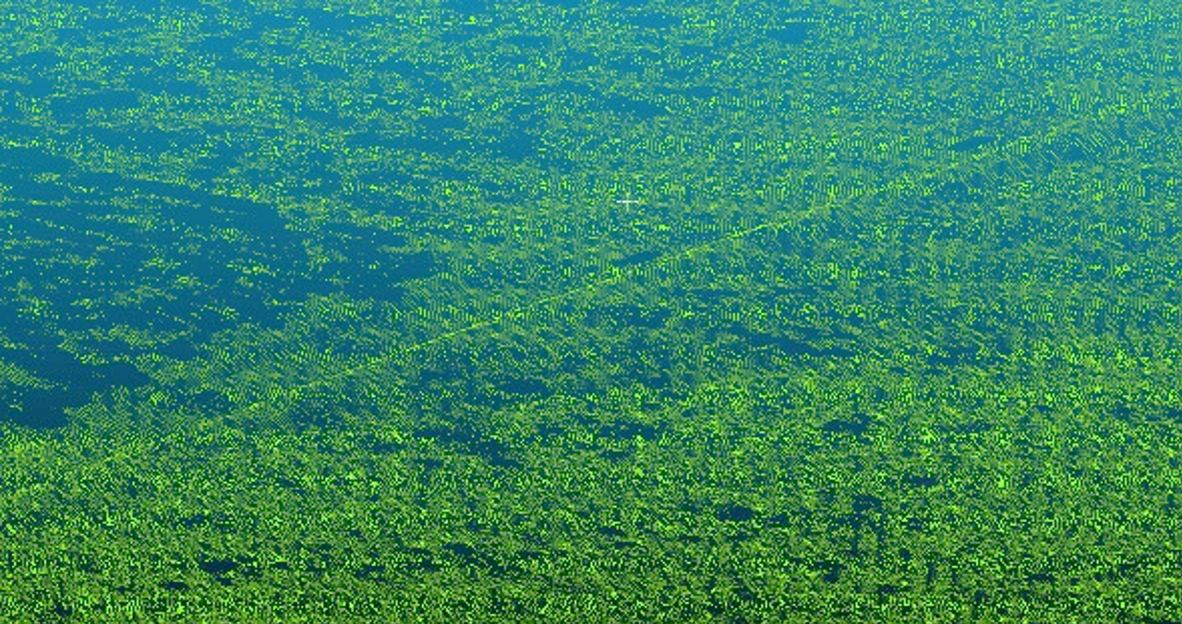
\includegraphics[width=6cm, height=3.5cm]{final_report/figs/ahn_sample_33CN2_a.png}} \\
Rotterdam Ketheltunnel, 37EZ1 & This segment of the A4 heading North from Rotterdam has been recently reconstructed in an underground tunnel. In addition, a significant portion of this R-road now runs in a trench towards Delft. AHN3 was imaged during the reconstruction, and hence contains anomalous data about the road surface. & \raisebox{-0.94\totalheight}{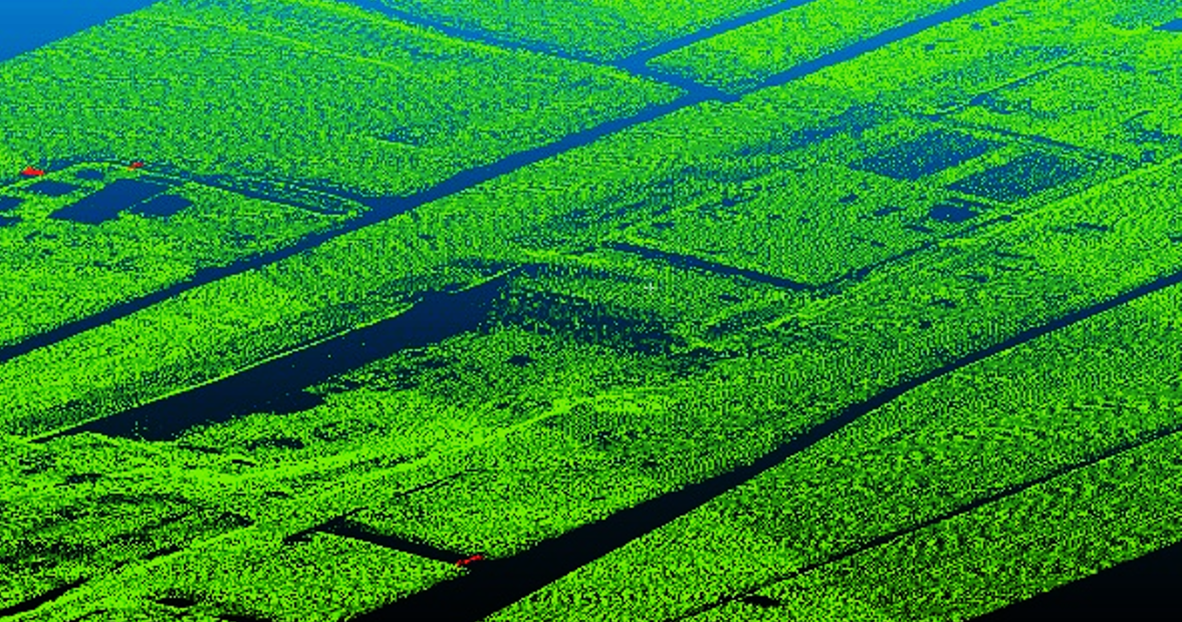
\includegraphics[width=6cm, height=3.5cm]{final_report/figs/ahn_sample_37EZ1_a.png}} \\
Knoppunt Ridderkerk, 37HN2 & The Ridderkerk interchange is one of the largest of its kind in The Netherlands, in one place containing 4 overlapping R-roads. Furthermore, it contains a high density of R-roads in a small area, many of them very tightly packed. Many of them have very sharp bends. & \raisebox{-0.94\totalheight}{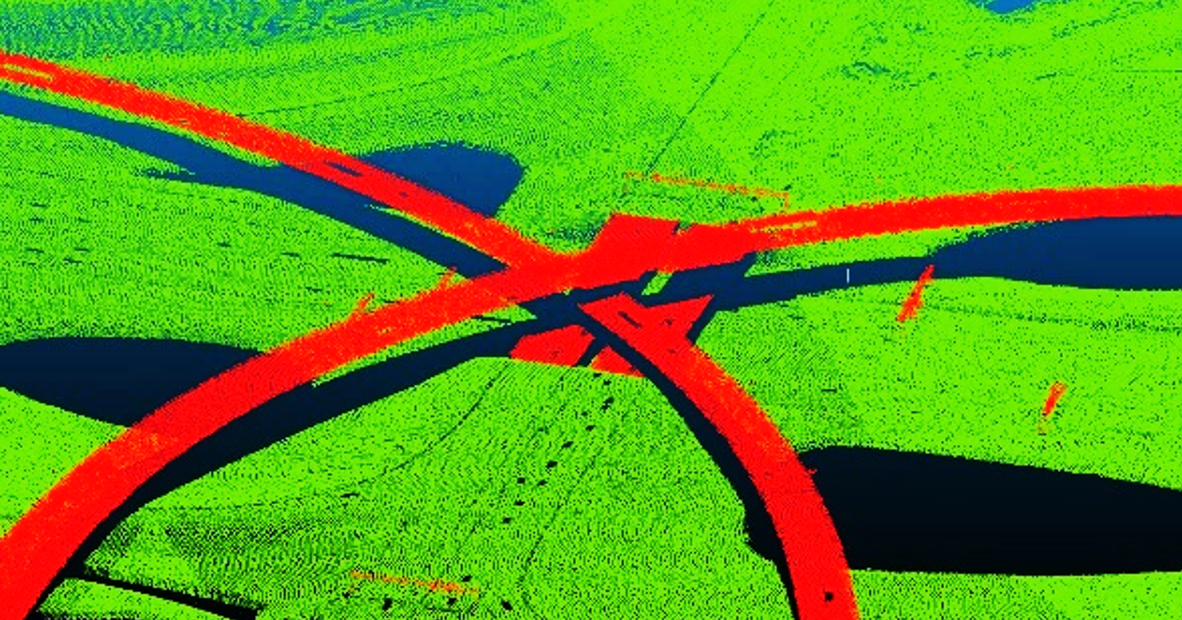
\includegraphics[width=6cm, height=3.5cm]{final_report/figs/ahn_sample_37HN2_a.png}} \\
Gorinchem, 38GZ1 & Complex interchange between a P-road and an R-road with small ramps, roundabouts and overlapping geometries. & \raisebox{-0.95\totalheight}{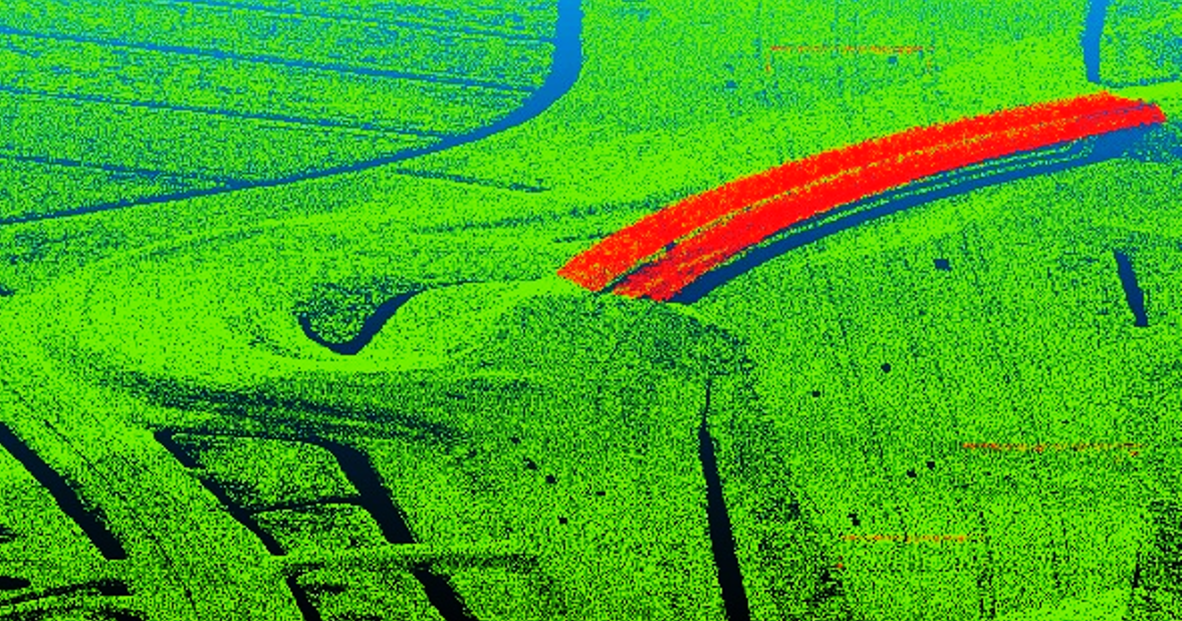
\includegraphics[width=6cm, height=3.5cm]{final_report/figs/ahn_sample_38GZ1_a.png}} \\
Knoppunt Deil, 39CZ1 & Less complex, but analogous interchange to the Knoppunt Ridderkerk. & \raisebox{-0.5\totalheight}{\textit{Please refer to Figures \ref{fig:ahnbridges}, \ref{fig:ahnsigns}, \ref{fig:ahnnwb} and \ref{fig:dtbahn}.}} \\
\toprule
\caption{Inventory of testing datasets \label{tab:inventory}}
\end{longtable}

One instance of my software can process a single testing dataset at a time. However, running multiple Python instances in parallel allows one to easily parallel-process multiple tiles depending on the CPU installed in the computer. Each dataset consists of a cropped NWB and DTB file, and the clipped AHN3 point cloud.

All datasets mentioned in Table \ref{tab:inventory} are part of the GitHub release of the results. A compressed archive with the input testing files (and all intermediate results and final results) can be downloaded via a link found in the repository's readme.

\section{Results of processing steps}
\label{sec:results}

The results below are presented in the same section structure as the detailed methods were in Section \ref{sec:methods} of the previous chapter. This is intended to make it easy for readers to correlate aspects of the results with details about the underlying processing steps. In each section, I describe - with the help of 3D visualisations - how well each processing step performs, and how effective and useful they are in the context of the entire pipeline as a whole. I also devote attention to describing typical scenarios in which algorithms are useful and perform well, as well as ones where the opposite is true and artefacts may be generated. Lastly, in each of the pipeline steps I make mention of how exactly the underlying software implementation is meant to be used, with notes on the recommended arguments.

\subsection{Splitting NWB into NBRS}
\label{sub:r_nbrsgeneration}

Each line colour in Figure \ref{fig:lidarsegmentation0} belongs to a specific NBRS, meaning that wegvakken that belong to the same NBRS are coloured the same. The figure illustrates that as a result of the NBRS generation step, the cropped road network becomes semantically enriched with identifiers linking certain LineStrings together, based on semantic or geometric conditions depending on which algorithm was used. The colours are generally inconsistent between the two visualisations because although the same colour scheme was used to prepare them, the two algorithms distribute the NBRS IDs themselves differently.

\subsubsection{Problems due to NWB intersection angles}

The figure also illustrates the fundamental differences that exist between the results of the two algorithms. The geometric algorithm makes the assumption that the 2D georeferencing of NWB is representative of the real-life geometry of road centrelines. However, I found this to be violated in various places as already mentioned in Section \ref{sub:nwb}. The problem relevant to these results is that wegvakken that represent a ramp merging onto a motorway lane or another ramp often end at abrupt angles, which can be observed in various places in Figure \ref{fig:lidarsegmentation0}. These angles are not representative of the real-life road geometry, they were drawn manually by data handlers to ensure that NWB complies with certain external requirements. Consequently, they may prevent correct decisions to be made based on the intersection angles, as a result.

\subsubsection{Example of issues with geometric algorithm}

In places where the above intersection angle related problem exists, choosing the straightest continuation across an intersection when building an NBRS does not necessarily represent the optimal choice, because the angles are artificial. This can be observed in the top half of Figure \ref{fig:lidarsegmentation0}, where I numbered some of the NBRS on the geometric results. While the geometric algorithm obviously made the right choice based on the pairwise angles between the individual road segments concerned, attribute table data told the semantic algorithm that the role and road number of certain parts of NBRS 0 and 2 are the same as that of NBRS 1, which resulted in these parts of NBRS 0 and 2 connecting via NBRS 1. The "discarded" ends of NBRS 0 and 2 then became two unique NBRS by themselves. In the overall large-scale context in this figure, the semantic algorithm evidently made the correct choice, even though this introduces some small, abrupt internal angles into the NBRS.

\subsubsection{Example of issues with semantic algorithm}

On the other hand, the red circle in the semantic NBRS generation results points out a place where the role and road number of a ramp changes suddenly, outside of a real-life intersection, which results in the algorithm abruptly starting a new NBRS there. The break happens in an unfortunate location, in the middle of a multi-level interchange where the continuation of NBRS is crucial so that large-scale trends across the complicated zone may be recognised effectively in later steps. This demonstrates that while the geometric algorithm is sensitive to problems with the georeferencing of the data, the semantic algorithm is sensitive to issues with the attribute table data. Within the testing tiles I examined, both algorithms offer an equal amount of benefits and drawbacks.

\subsubsection{Evaluation and choice of algorithm}

Both algorithms produce useful, if not perfect, results. In general, the resulting chains of wegvakken (LineStrings) satisfy all the original requirements I set for the outputs of this step (minimise internal angles, maximise length, disallow self-intersections and branching). Based on some further testing after implementing the rest of the pipeline, I also verified that the choice of algorithm does not significantly influence the output of subsequent steps. Since the geometric algorithm generalises to arbitrary road networks better than the semantic algorithm, I used it to generate the rest of the results shown and discussed in the present chapter.

\subsubsection{Using the implementation}

In the software, before NBRS generation can be executed, the \codeword{nbrs_manager} class needs to be initialised with the file part to the cropped NWB file of the desired dataset. By default, the software uses the geometric algorithm, but an optional argument is provided to switch to the semantic one. Example calls to perform semantic NBRS generation are provided below.

\begin{lstlisting}
roads = nbrs_manager(nwb_fpath)
roads.generate_nbrs('semantic')
\end{lstlisting}

In the code snippet above, \codeword{nwb_fpath} refers to a variable containing the file path in the operating system to the cropped NWB file of the desired testing dataset. For instance, the file path could end in \codeword{.../C_39CZ1_nwb.shp}, using the naming convention of the released testing files, the dataset called "Knoppunt Deil" is desired. The modules numpy, GeoPandas and shapely need to be imported before running NBRS generation, and the shared library \codeword{lib_shared.py} also needs to be imported. The code \codeword{roads.plot_all()} may be executed to plot the results on a 2D diagram using random colours to distinguish between NBRS. At this point, NBRS generation results are saved in class variables only (see \codeword{roads.nbrs_wvkn}), hence running \codeword{roads.write_all()} at this point is \textbf{not} going to write the NBRS IDs into the attribute table.

\subsection{Elevation estimation}
\label{sub:r_elevationestimation}

Figure \ref{fig:elevationestimation0} shows the results of this step in two 3D visualisations. The NWB centrelines are shown once again in random colours based on which NBRS they belong to, but now they are shown at their estimated elevations. The vertical dimension in this visualisation is exaggerated 5-fold, so that changes in elevation are better visible. The figure contains two visualisations, so that more features are made visible that I discuss in the next paragraphs, and to allow the reader to examine the same results from multiple viewing angles.

\subsubsection{Vertex densification}

The vertices have already been densified at this point, I used a threshold of 5 metres for the final outputs shown here. This means that no individual line segment in the 3D road network is longer than 5 metres. I found this threshold value to offer a compromise between longer processing times and more refined results, and to work well with subsequent processing steps. The polynomial fitting step of the elevation estimation procedure already made use of the additional vertices, hence we may say that while the horizontal dimensions were merely oversampled, the vertical dimension benefited from the vertex densification in the sense that it is far more detailed than it would be without the added vertices (as also mentioned in Section \ref{sub:m_elevationestimation}). An example visualisation of what happens to a specific NBRS during vertex densification is shown in Figure \ref{fig:elevationestimation1}.

\subsubsection{Types of challenging scenarios}

I will keep the description of these intermediate results brief, as the comparison with the final results in Section [REF] contains an in-depth description of them. Instead of going into details, I will focus on the general quality of the results, also because accuracy is not yet important at this step - this 3D conversion is merely a stepping stone towards the goal of performing Lidar segmentation.

The are two main aspects of the output that require our attention: how close to the real-life surface of the road the 3D centrelines are being shown (effectiveness of the 3D conversion), and how succesfully positive outliers are being eliminated (effectiveness of the refinement step). The former can be assessed via visual comparison with the underlying AHN3 point clouds, while the latter can be examined by looking for artefacts at locations where occlusion happens. Figure \ref{fig:elevationestimation2} shows two further 3D visualisations that contain examples of the features that are relevant for this assessment.

\subsubsection{Effectiveness of 3D conversion}

The visualisation on the left illustrates that in the case of flat lengths of roads, centrelines are generally positioned very close to the Lidar-defined road surface (within a few centimetres in general). Outliers are atypical in well-exposed areas, corresponding to the lack of outliers in AHN3 itself (and its ground classification). The procedure is fast, runtimes for the testing datasets are generally in the range of 5 to 30 seconds on a mediocre computer.

Thinning the input point cloud aggressively may marginally improve the performance of this step, but it drastically reduces its effectiveness in areas that are poorly sampled. This in turn may result in artefacts on a scale that also confuse the refinement step. I found that working with no thinning applied, or a maximum factor of 3 (33\% of points kept) at most, works best. My final configuration uses a thinning factor of two while it imports the AHN3 data, which is carried over to all subsequent steps that work with Lidar data.

There is a range of factors that may result in the computation of anomalous preliminary elevations due to occlusion. Firstly, if an NWB centreline is positioned far from the actual road centreline (or next to the road), then the 3D elevations will be derived from a patch of Lidar points that may include a significant number of off-road points, which may result in both positive and negative outlier elevations. Furthermore, bridges in AHN3 include reflections from civil engineering structures, which are often attached to roads close to their edges. If the centreline of an NBRS falls too close to the edge of the road where such objects are present, its elevations may be corrupted by Lidar points reflected from them, rather than from the road surface.

Furthermore, slow or stationary vehicles and motorway signs, and larger occluding objects (e.g. bridges built \textit{over} a given road) tend to generate a sequence of outlier vertices, depending on the size of the object. Vehicles generally represent an issue in this step only on bridges, as on bridges they form \textit{part of} the bridge classification of AHN3, and are thus retained in our input - however, the \textit{gaps} left by filtering out vehicle reflections may occasionally mean that no points can be obtained within the query radius, resulting in a missing elevation. Overlying bridges present the most pervasive issue in terms of their frequency of occurrence. The outlier elevations and missing elevations resulting from these artefacts are mostly eliminated by the refinement step (see below).

The query radius used in the KD-tree queries in my final configuration is 1 metre. At the typical local posting distances found in AHN3, this allows the algorithm to fetch enough points even when vertices are close together, but does not generally include off-road points. This query radius corresponds to a query area of $\pi$, containing a typical amount of 10-15 AHN3 points assuming a thinning factor of 2 was used. When vertices are sparser (a higher thershold was used in vertex densification), a slighly higher radius is recommended, as it allows the program to sample a larger area of the road surface to make up for the decreased amount of vertices, bearing in mind that a much larger radius may result in too many off-road points being considered.

\subsubsection{Effectiveness of refinement step}

The benefits of the refinement step are made evident by the shape of the 3D centreline shown on the left in Figure \ref{fig:elevationestimation2}. The road passing over the other causes occlusion, meaning that Lidar data is unavailable for the surface of the lower road for a short distance. Before the refinement step, the centreline of the lower road thus becomes snapped to the elevation of the one above. The outliers introduced due to this are then easily identified and eliminated by the refinement step, and new values are interpolated based on the polynomial model that was fitted on the NBRS.

For my final outputs, I used a degree of 12 for the polynomials, and set the outlier filtering threshold to 0.2 times the standard deviation of the data-model errors in the given polynomial fit. I found that in general these work best with the testing datasets. Decreasing the vertex densification threshold and increasing the polynomial degree allows one to use lower filtering thresholds, and 0.2 works well with my final parametrisation. Standard deviations below 0.4 metres are artificially icreased to 0.4 metres to avoid modifying most elevations in roads whose conformance with the model was found to be near-perfect. More information about the detailed processing (and thus, the exact way in which these parameters are used) in Section \ref{sub:m_elevationestimation}.

This approach proved to be an effective solution to eliminating occlusion-related artefacts, it is ineffective only in places where the occluding geometry is close to the road surface. For instance, stationary vehicles occasionally introduce outliers that are not far enough from the model to be fetected in the refinement step, thereby giving rise to small spikes in the output. This does not happen frequently, and does not represent a problem in the context of the pipeline as a whole. This step also solves the outliers generated by motorway signs, which are high enough above the road surface to be detected as such. A lower limit for the outlier filtering threshold is set, in practice, by the accuracy of the polynomial fits themselves. If the limit is set too low, elevations may be replaced that were in fact correct, but which represent geometric features that the polynomial cannot approximate well.

The above issue also causes further problems where the vertical curvature of roads is unusually high, such as in the overpass shown on the right in Figure \ref{fig:elevationestimation2}. Such curvature is difficult to approximate using polynomials, especially if the corresponding NBRS is long and thus contains other types of curvature too. In such cases, the refinement part of the algorithm may erratically identify lengths of such roads as outliers and reposition them at the lower elevation level set by the polynomial model - even if the outlier detection threshold is sufficiently high. I successfully bridged this issue by implementing workarounds in the Lidar segmentation workflow. Therefore, these inaccurate elevations do not represent a problem on the scale of the pipeline as a whole. Shorter NBRS lengths could help deal with this issue in a more explicit manner, but this would also mean that certain longer trends would become impossible to model later on.

\subsubsection{Using the implementation}

The below code snippet shows the code I used to generate my final results.

\begin{lstlisting}
roads.densify(5)
roads.estimate_elevations(ahn_fpath, r = 1, thin = 2)
roads.write_all(simpleZ_fpath)
\end{lstlisting}

The first line performs vertex densification with a threshold of 5 metres. The second line performs the preliminary elevation estimation (and refinement) step, the variable \codeword{ahn_fpath} is assumed to contain a file path to the clipped AHN3 file belonging to the current testing dataset. For instance, it could be \codeword{.../C_39CZ1_2_26_clipped.las} using the naming convention used in the input files I released on GitHub. The tags \codeword{_2_26_clipped} in these file names refer to having kept only points in classes 2 and 26 (ground and bridge points respectively), and having clipped it to the extents of buffered centrelines. The variables \codeword{r} and \codeword{thin} control the query radius and thinning factor respectively, their default values are shown above.

The last line of code writes the resulting 3D geometry to disk, "mimicking" the semantic and geometric structure of the input file. The variable is named in such a way to distinguish it from the variable containing the file path where the end results are written, called \codeword{accurateZ_fpath}. This step is not compulsory, it is intended for debugging and demonstration purposes only. I will list similar commands for subsequent pipeline steps, where the same applies - intermediate results are stored in the class and thus subsequent pipeline steps have access to them without the need to write them to files.

In the class itself, the results of this step are not stored in a separate variable, but are added to the GeoDataFrame representation of the input NWB Shapefile. This can be found in the \codeword{.nwb} variable of the \codeword{nbrs_manager} class.

\subsection{Lidar segmentation}
\label{sub:r_lidarsegmentation}

Figure \ref{fig:lidarsegmentation0} shows some visualisations of the results of Lidar segmentation. Like in figures depicting NBRS alone (such as e.g. Figure \ref{sub:m_elevationestimation}), I used colours to dinstinguish between NBRS. In this figure, I coloured those Lidar points the same, which belong to the subcloud of the same NBRS. The NBRS themselves are all shown in black to help distinguish them from their subclouds. For subclouds which are positioned far from each other, a clear separation is observable. However, ones that are close to one another often overlap (such as on the left in Figure \ref{fig:lidarsegmentation0}), which is the result of there not being much space between the roads themselves that the underlying NBRS represent. The overlapping parts of such subclouds may contain duplicate points (in other words, points may be part of several subclouds). The visualisation only shows the ones that were loaded last, hence some subclouds may appear thinner in the visualisation than they really are.

\subsubsection{General description of results}

The properties which we are looking for in the resulting subclouds, is that they contain as many of the road surface points, and as few of the surrounding unrelated points, as possible - especially with regards to points reflected from occluding objects. Figure \ref{fig:lidarsegmentation0} illustrates quite vividly that indeed, each NBRS's subcloud is clearly related to the underlying real-life road surface and that almost no unrelated points are included.

Since this is not yet the stage where conservative thresholds are being enforced, it is possible that next to the road surfaces, some parts of the AHN3 cloud will be retained that represent slopes or other surfaces \textit{next to} roads, rather than the roads surfaces themselves. This is especially prominent before and after regions of occlusion, where the underlying plane fits have already been affected by the occlusion, but not enough to be excluded. Some examples of such areas are shown on the right in Figure \ref{fig:lidarsegmentation0}. Since the Lidar patches inevitably include off-road points, the fitted planes will not lie perfectly on the road surface, in turn causing the inclusion of these undesired points in the output. This step of the pipeline is not yet concerned with eliminating these, this is one of the purposes of the edge approximation, edge optimisation and conditional TIN construction pipeline steps that come after this step.

The visualisations in Figure \ref{fig:lidarsegmentation0} show the Knoppunt Ridderkerk motorway interchange in which many motorway lanes and ramps are present in complex 3D relationships, in one place including an area with 4 overlapping roads. The correctness of the resulting subclouds demonstrate that although some of my approach is procedural and relies on a fixed parametrisation, it is still robust enough to work in the simplest, as well as the most challenging scenarios.

\subsubsection{DTB's usefulness}

The final version of my code can navigate through long occluded regions without DTB coverage, but DTB is still used wherever available and useful. Unlike in most locations, DTB has good coverage in the particular motorway interchange shown in Figure \ref{fig:lidarsegmentation1}. The visualisation on the right shows how this manifest itself in the output. Where subclouds contain Lidar gaps filled with points in a linear arrangement, one can be certain that DTB was called on to re-fit planes and supply points to the output.

Not only does this help the algorithm keep its plane fits stable through regions of occlusion (thereby producing a more accurate subcloud from AHN3), it also represent the only source of data in regions where AHN3 is completely missing. Without these data points, later part of the algorithm would need to interpolate elevations based solely on information from outside of the data gap, leading to a drastic drop in confidence.

While this demonstrates that DTB - or any support dataset with road surface elevation measurements - can be helpful in complementing this procedure (which is otherwise based entirely on AHN3), it also highlights some of DTB's weaknesses. While this area has good DTB coverage, the DTB lines in some parts of the interchange are approximately two decades older than the AHN3 measurements. As one can see in \ref{fig:lidarsegmentation1}, there are noticeable systematic differences between the road elevation as depicted by AHN3 and DTB, which is not seen everywhere, especially not in regions where the temporal offset of DTB is not so large. I suspect the primary reason for this 0.2-1 metre difference to be regional subsidence.

This, in turn, points towards the wider issue of the temporal discrepancy between all our datasets, which is further discussed in Section [REF].

\subsubsection{Splitting NBRS into parts}

On the left in Figure \ref{fig:lidarsegmentation2}, a region with neither AHN3, nor DTB coverage is shown. In this location, the NBRS was split into two parts and in the figure, this is illustrated by the fact that I could highlight the subcloud on one side of the gap separately. The matching colour of the points show that they still belong to the same NBRS, but the program stores a separate subcloud for each NBRS part, meaning that they are loaded as a separate MultiPoint object in the 3D viewer I used to generate these figures.

NBRS splitting works well in general, and it ensures that useful subclouds are generated wherever it is possible to generate them - regardless of what other, challenging features may be present in a given NBRS. In Section [REF] this is further discussed in the context of tunnels.

\subsubsection{Parametrisation}

The parametrisation of this pipeline step is extensive, because many parts of the algorithm are of a procedural nature. Hence, I will dedicate some attention here to describing the final parametrisation I used to produce my outputs. Here I will not go into details about the exact way in which these parameters are used, as I have already described this in Section \ref{sub:m_lidarsegmentation} without specifying numerical values. All parameters were derived from a process of experimentation and fine-tuning, although a good understanding of the issues, the procedures and the properties of the input data were also essential in being able to define the parameters and find suitable values for them.

Firstly, a query radius needs to be specified, which requires some fine tuning, so I exposed it as an argument of the class method in the implemetation, that handles this pipeline step. I used a query radius of 10 metres, which is sufficiently long to allow most of road surface reflections to be included between centreline vertices. Using a smaller radius could, in some cases, improve the plane fitting results, but it would also cause the exclusion of useful Lidar points from the patches simply due to the spherical geometry of the query regions. Due to performance considerations, I did not implement a custom query mechanism - the performance of the radial KD-tree queries is certainly required for this step. The performance of this step is also heavily affected by the vertex densification threshold and thinning factor used previously; denser NBRS vertices and a denser input point cloud means that the processing time will increase considerably.

When the program examines the Lidar patches corresponding to each NBRS vertex, it either fits a plane and passes on the patch, only passes on the Lidar patch, or does neither. Two separate thresholds govern this behaviour, and both are defined in units of points per square metres. The program stops fitting planes below 2 points per square metre, and stops passing on points below 1. In this context, "points per square metre" is interpreted rather loosely, since the patches are actually based on points falling into spheres of a given radius rather than circles. However, since Lidar points are expected to have been reflected from a \textit{nearly} 2.5D surface, this assumption is not unreasonable. In fact, I defined the parameters in such a way, that they can be easily correlated with the specifications of AHN3, which also uses this unit (see Section \ref{sub:ahn}).

The following set of values controls the detection of instability when examining the succession of plane fits and underlying Lidar patches. DTB-based assistance is attempted if any of the following conditions are met: the standard deviation of the Lidar patch's elevations exceeds 0.1 metres, the distance between the plane and the corresponding NBRS vertex grew by more than 50\% since the previous iteration, or median of the Lidar patch's elevations grew by more than 50\% since the last iteration. The latter two conditions are only considered if the absolute value of the underlying metrics (distance from NBRS, median elevation) exceeds 0.2 metres.

When DTB-based assistance (re-fitting of plane) is attempted, the initial query radius when looking for DTB points is 0.4 metres. If enough points were found to re-fit the plane (more than two), then the second repositioning query is performed with the same radius as the one used in the generation of the Lidar patches (10 metres in my final parametrisation), because at this point it is assumed that the query position has been moved relatively close to the true elevation of the road surface. When deciding whether to do a final re-fit on the nearby part of the Lidar patch, the program once again uses the condition that the density of these points should at least be 2 points per square metre. Lidar points are deemed to be close if they are less then 1 metre away from the plane, which is defined as 10\% of the Lidar patch query radius in the code.

When pre-selecting the final set of conformant points from the patches, the program uses a threshold of 5\% of the query radius used in the Lidar patch queries, corresponding to 0.5 metres in my final parametrisation.

While the post-processing operations of this pipeline step (breaking into NBRS parts and filtering outliers) also have a few parameters, these are insignificant and are thus omitted from this discussion.

\subsubsection{Using the implementation}

The below code snippet shows the code I used to generate my final results.

\begin{lstlisting}
roads.segment_lidar(dtb_fpath, 10)
roads.write_subclouds(subclouds_fpath)
\end{lstlisting}

The first line performs the point cloud segmentation itself, with a radius of 10 metres for the KD-tree queries that generate the Lidar patches. The variable \codeword{dtb_fpath} is assumed to contain the file path to the cropped DTB file belonging to the desired testing dataset. The second line writes the resulting subclouds to disk, the argument variable is assumed to contain the file path to the desired output file.

The intermediate result that the second line writes to disk "mimics" the structure of the input LAS file. However, each point is given three new properties. The property \codeword{ORIGIN} determines whether the given point originates from AHN3 (denoted by the value \codeword{0}) or DTB (denoted by the value \codeword{1}). The properties \codeword{NBRS_ID} and \codeword{PART_ID} determine which NBRS, and which part of that NBRS a given points belongs to. NBRS that were not split into parts are still represented by the same data structure, but all their points are found in a single part with ID 0.

In the class itself, the resulting subclouds can be accessed via \codeword{.nbrs_subclouds[nbrs_id][part_id]}, where \codeword{nbrs_id} and \codeword{part_id} are variables which should contain the ID of a specific NBRS, and the ID of one of its parts respectively. Furthermore, one can find the indices corresponding to intervals with AHN3 or DTB coverage in \codeword{.nbrs_parts[nbrs_id]}, which effectively defines the NBRS parts.

\subsection{Edge approximation}
\label{sub:r_edgeapproximation}

Visualisations showing the results of the edge approximation step are shown in Figure \ref{fig:edgeapproximation0}. The black lines correspond to NWB centrelines, while the closely spaced, orthogonal lines are the cross-sections that are attempted to be created on each vertex (including those resulting from densification). The lines connecting the ends of the cross-sections on each side of each centreline are the preliminary edges that are the main product of this processing step. The vertical dimensions is once again exaggerated five times, make elevation differences better visible.

\subsubsection{General description of results}

The edges generated in this step are mostly according to my expectations. Owing to the verification step that takes place before accepting a cross-section (and extending the preliminary edge with its end vertices), the general shape of the edges is quite well-behaved, and their elevation reflects what one would expect based on the underlying subclouds. In my final configuration, cross-sections have vertices every 10 centimetres (created via densification), and their elevation is derived from points no further than 25 centimetres away. This dense quantisation allows the algorithm to reconstruct road edges on a fine scale.

On the left in Figure \ref{fig:edgeapproximation0}, I visualised the preliminary edges only, while on the right I attempted to create a visualisation in which the preliminary edges and cross-sections can be compared to the subcloud that was used to generate them. While the overall quality is good and the results are certainly usable in terms of the requirements of the next two pipeline steps, there are a few limitations and problems that are worth discussing.

\subsubsection{On road width bounds}

As I already mentioned in Section \ref{sub:m_edgeapproximation}, the algorithm works with a fixed minimum and maximum road width. The maximum is enforced by using it as the length of the constructed cross-sections, while the minimum is enforced as part of the verification step.

The enforcement of the minimum width is less of a limitation; it merely prevents the cross-sections from shrinking too short. However, the the way in which the maximum width is enforced can be considered a limitation because road surfaces that are unusually wide will not be included in their entirety. Using very long cross-sections increases the chances of returning false hits due to short successions of off-road points that conform well with the overall trend in the linear regression of the cross-section. With shorter cross-sections, the chances of this happening are reduced drastically. My final parametrisation has a minimum and maximum widths of 3.5 and 7 metres respectively. Most of my testing tiles contain relatively wide roads, for thinner roads I recommend reducing these parameters, which are exposed as arguments in the software.

While the maximum limit may exclude meaningful road surface areas in the case of unusually wide roads, there are special roads in which a sudden break in the surface cannot be used to detect their edges. Motorway lanes are represented by discrete centrelines in NWB, which means they will be treated as individual roads in my model. However, such lanes are often constructed on a single paved surface, meaning that my method cannot be used to derive edges between them. This is another reason why the maximum width is important, and one such scenario is shown on the left in Figure \ref{fig:edgeapproximation1}.

A circumstance that necessitates the use of a lower value for the maximum width is the main problem with NWB's georeferencing: if NWB itself is shifted towards the edge of a road locally, generated cross-sections will be corrupted there by off-road elevations. Using larger values for the maximum width will only make this problem worse. In the absence of this problem, the value could be increased by a few metres based on my experience with accurate parts of NWB. The feature that the line fits can be fitted only on the central portion of cross-sections was developed specifically to mitigate the effects of this issue, and in my final configuration the central 40\% of the cross-sections is used for this.

\subsubsection{Failed edge detection}

While in well-exposed, straight roads this does not generally happen, there are lengths of roads where finding edge points will fail repeatedly. In such places, the algorithm does not save the cross-section, and also does not add edge points to the preliminary edge LineStrings. One the left in Figure \ref{fig:edgeapproximation0}, this can be clearly seen by the gap in cross-sections. In There are various reasons why this might happen, which I will discuss below.

The most common reason is the lack of data. If not enough Lidar points are found close to the cross-sections, then the line fits will not be constructed and the algorithm will skip to the next vertex of the NBRS part. This happens in data gaps where both AHN3 and DTB are missing, and also in most gaps where only DTB is available. The latter is due to the fact that DTB samples linear features along the length of each road, and has a poor sampling rate in the direction that the cross-sections are attempting to sample as a result. Such data gaps may exist under bridges for instance, but also in places where vehicles occluded a significant portion of the road. The latter also causes abrupt width changes, which may be accepted by the algorithm if it happens when the conditions are relaxed due to repeated failures. This can be seen on the right in Figure \ref{fig:edgeapproximation1}.

The second most common reason is the construction of anomalous plane fits. If the elevation estimates of the cross-section vertices are scattered, the errors in the fit will be large. Elevations further than one standard deviation of the data-model error are not considered any further, and many points are filtered out in such a way, the cross-section will be abandoned and the software will skip to the next one. This could be due to various reasons. By far, the most common one is the misalignment of NWB with respect to the real-life centreline, which results in the inclusion of both road, and off-road elevations in the cross section, leading to a poor fit. Other reasons include the presence of Lidar reflections from above the road surface (from vehicles or bridge structures), as well as problems with the line fits due to unusually thin roads.

Lastly, failures may also be the result of violating the conditions of the verification step. Namely, if the width would be too thin, or if a unrealistically sudden width or elevation change is detected. If this is the sole reason for the failures, then generally only a limited number of cross-sections and corresponding edge vertices will be missing, as the conditions are relaxed after 3 successive failures.

\subsubsection{Artefacts in zones of missing data}

In the absence of AHN3 data, vertices will be skipped, as I mentioned above. However, quite frequently, one or two cross-sections will be accepted in such regions too, if AHN3 coverage reappears temporarily, for instance due to a small gap between two bridges. Due to the repeated skipping of vertices, the conditions will almost certainly be relaxed by this point, and hence a sudden width or elevation change will be allowed. This combination of factors may result in strange edge geometry being generated in zones of occlusion. This is one part of the pipeline which benefited from being able to split NBRS into parts - not having to work with such zones helps avoid the generation of corrupted preliminary edge geometries, improving edge quality close to these zones of occlusion.

\subsubsection{Using the implementation}

In my example code on GitHub, I use the following two lines to generate and export the preliminary edges:

\begin{lstlisting}
roads.estimate_edges(min_width = 3.5, max_width = 7, thres = 1, perc_to_fit = 0.4)
roads.write_edges(edges_fpath, crosses_fpath)
\end{lstlisting}

The first line generates the preliminary edges. The arguments (all compulsory) set the minimum and maximum road width, the outlier filtering threshold, and the ratio of how much of the cross-sections should be fitted with lines. The first two arguments should be specified in metres. The second argument specifies the number of standard deviations of data-model errors, within which points should be considered inliers, so the current value means one standard deviation. The last argument accepts values between 0 and 1, the current value means that the central 40\% of cross-sections will be used as the basis for the line fits (even if it will then be used for comparisons outside of this reduced length via extrapolation).

The second line writes the results to disk. Both the edges and the cross-sections are written, \codeword{edges_fpath} and \codeword{crosses_fpath} are assumed to contain file paths where these should be written (as Shapefiles). In the class itself, the results are found in \codeword{.nbrs_edges} and \codeword{.nbrs_crosses} as GeoDataFrame objects.

\subsection{Active contour optimisation}
\label{sub:r_activecontours}

As Figures \ref{fig:activecontouroptimisation0} and \ref{fig:activecontouroptimisation1} show, all planned parts of this pipeline step output the expected results, albeit with occasional artefacts and a mediocre overall quality. The contours are smooth, they generally reflect the shape of the roads accurately, and only occasionally suffer from major blunders. However, even small deviations towards beyond the edge of the roads mean that based solely on these contours, off-road Lidar reflections would be classified as road points and thus be inserted in the TIN model in the next step. Unfortunately, small such deviations occur frequently, as the close-up images in Figure \ref{fig:activecontouroptimisation1} demonstrate. With the help of the results, this section will focus on explaining why exactly it is difficult to guarantee that this workflow functions reliably, as this was the reason for a major revision of the design of the preliminary edge detection and TIN construction steps, which I already explained in Section \ref{sub:m_edgeapproximation}.

\subsubsection{Attractor maps}

Some attractor maps can be seen in Figure \ref{fig:activecontouroptimisation1}. Each NBRS part has its own attractor map, and since subclouds may overlap, so can the attractor maps. In the figure, attractor maps that are separated from others by a fair amount of distance can be examined in their full width, while only the one the was drawn last by the visualisation software can be examined in its full width, where overlapping occurs. The bright parts of the attractor maps correspond to regions were the normal vectors of the surface are oriented uniformly, while the darker regions indicate divergent normal vectors. The linear boundary between such regions thus marks the edge of the smooth road surface in most places, as it corresponds to an increase in normal vector divergence. I used a pixel size of 0.5 metres (in both dimensions) to generate these attractor maps, and the attractor map values are based on using a 5-by-5 kernel, assessing correlation in the neighbourhood via approximately 30 inner products for each pixel.

The optimised contours are shown overlain on the attractor maps on the right in Figure \ref{fig:activecontouroptimisation1}. While the \textit{general} appearance of the contours is acceptable, comparing \textit{details} in the contours with the attractor maps reveals that the contours are in fact not reliably positioned on the break in smoothness. So that the reader can better interpret the optimisation as a process, the left part of Figure \ref{fig:activecontouroptimisation1} shows the preliminary edges overlain on the attractor maps. Comparing the preliminary edges to the contours in the context of the attractor maps allows one to better understand the effects of the optimisation procedure. In particular, patterns in the behaviour of the optimisation procedure may be recognised.

\subsubsection{Patterns of failure}

One important pattern is that the contours are sensitive to small-scale features in the preliminary edges. A few outlier edge points (an short, abrupt expansion of the preliminary edges, for instance) can introduce large bulges into the optimised edges. Similarly, where the preliminary edges shrink (for instance due to the influence of stationary vehicles), the optimised contours will tend to do so too, but on a much larger scale. In general, small "horizontal outliers" in the preliminary edges tend to become vastly exaggerated during optimisation.

Another pattern, which I already mentioned in \ref{sub:m_activecontours}, is that where preliminary edges fall outside the bright part of attractor maps, the the optimisation procedure will often fail to draw them back to the primary break in smoothness. The off-road parts contain various other high-contrast features due to the unevenness of the underlying real-life surfaces, and the edges will often be drawn to some of these instead of the edge of the road. This is in part due to the large weight the optimisation algorithm gives to the \textit{proximity} of the edges. Due to this, deliberately underestimating the road width does not represent a solution: if the preliminary edges are too far inwards from the break in smoothness, they will simply stay in their original position during optimisation, rather than be drawn to it. This behaviour cannot be changed simply via the parametrisation - I already give nearly full weight to edge detection in my final configuration, over attraction to brightness or darkness. I also experimented with the other trivial approach, i.e. deliberately underestimating the preliminary road width and giving more weight to attraction to darkness in addition to edge detection. Unfortunately, the results of this approach are even more unpredictable.

Lastly, the contours may also become corrupted by the break in smoothness itself missing from the attractor maps. This circumstance may arise as a result of various real-life features. The two most common reason are the paved surface being unusually wide (wider than the maximum width of the underlying point cloud), and AHN3 coverage being unavailable. The former is manifested in the attractor maps by the bright zone extending all the way  to the edge of the map. In such regions, active contour optimisation will mostly leave the preliminary edges largely unchanged (there are not edges to attract it), except when the edges are moved unusually far from their original position outward, which could be due to the second pattern I described above for instance. This combination of factors may introduce unpredictable artefacts into the results. No-data regions tend to cause unpredictable results for the same reason.

One aspect that deserves a mention is the handling of no-data pixels in the maps. The optimisation algorithm has no concept of empty pixels, all pixels need to contain a scalar value - finding a suitable one was thus a matter of experimentation. I found it most effective to set all no-data pixels to a value close to the one corresponding to the smooth road surfaces. While this creates a second, artificial break in the brightness of attractor maps (at the edges of the underlying subclouds), this proved to affect the results only to a small degree. On the other hand, it solved problems with occluded (missing) parts of roads - since no edges are created \textit{on} the road surface, the optimisation algorithm is much less likely to create sudden artefacts at these locations.

\subsubsection{Parametrisation}

As I mentioned above, I used a 0.5-metre pixel size for the attractor maps and about 30 pairwise inner products per pixel, to generate the attractor map's scalar pixel values. The details of the active contour optimisation algorithm's parametrisation are described in \ref{sub:m_activecontours}, here I will omit such a desription and focus on the choice of values instead.

The most important parameters in my experience are the two parameters that control attraction to brightness and edges. Both values can range between -1 and 1, corresponding to fully repelling and fully attracting the contour. In my final configuration, brightness and edge attraction are set to 0.05 and 1 respectively. This means that the contours will be very slightly attracted to bright regions, but mostly their iterative refinement will be governed by attraction to edges, for reasons I already discussed in the paragraphs above.

A parameter $\beta$ controls the smoothness of the resulting contours, which can also be intuitively though about as controlling the tension of the underlying splines that active contour optimisation repeatedly fits. I set this value to 0.01, which in my experience corresponds to medium tension. This helps minimise the effects of the types of issues I already described above by keeping the contour relatively tense across them, such as across small artefacts in the preliminary edges. 
For the $\alpha$ parameter (which controls lengthwise shrinking), I set a value of zero to indicate that this behaviour is undesired. I also found that giving the algorithm about 1000 to 5000 iterations to work with (rather than a strict termination condition) works much better. This number of iterations allows the contours to evolve sufficiently, but prevents artefacts from becoming too exaggerated, which happens rapidly if more iterations are allowed.

The time step $\gamma$ and the number of pixels the contours is allowed to shift in a single iteration can be used to further fine-tune how quickly the optimisation lets the contours evolve. I these two values to 0.005 and 1 respectively, which corresponds to a relatively slow iteration, appropriate to the small-scale changes we desire (generally, we wish to move the edges only by up to a few metres.

The above parametrisation is the result of a process of iterative combined revision of the parameter values and the attractor map generation technique, as I mentioned in Section \ref{sub:m_activecontours}. While I have experimented with a wide range of parametrisations, the possibility remains that a better configuration exists. However, I was unable to find one within the amount of time reserved for this part of the project, leading to my decision to focus on improving preliminary edge estimation and making TIN construction more versatile. Furthermore, the combined computational complexity of generating high-resolution attractor maps using my technique, and that of the optimisation algorithm, meant that testing incremental changes is a rather difficult process.

\subsubsection{Choice of algorithm}

Contributing to the above uncertainty regarding the effectiveness of active contour optimisation is the fact that in relevant literature (e.g. \cite{boyko_funkhauser_2011}), mentions of its ineffectiveness relative to more sophisticated algorithms is made. My hypothesis was that with a sufficiently good pre-selection of Lidar points and pre-processing of attractor maps, conventional active contour optimisation would still work well, but this appears not to be the case reliably. Lesser known approaches, such as ribbon snakes (a sophisticated offshoot of active contour optimisation), exist but do not have open-source implementations. Considering the volume of further tasks in this project, I opted not to attempt to implement it based on first principles, especially considering that its superiority is not clearly demonstrated in relevant literature.

\subsubsection{Using the implementation}

The following lines of code may be used to run active contour optimisation and export the attractor maps and resulting optimised edges:

\begin{lstlisting}
roads.optimise_edges(size = 0.5,
                     a = 0, b = 0.01, g = 0.005,
                     w_l = 0.05, w_e = 1,
                     max_iter = 1000)
roads.write_maps(maps_fpath)
roads.write_contours(conts_fpath)
\end{lstlisting}

The first argument \codeword{size} in the active contour optimisation method corresponds to the desired pixel size. The rest of the parameters expose some of the active contour optimisation parameters that I found the be useful for making smaller changes to the algorithm's behaviour. The arguments \codeword{a}, \codeword{b} and \codeword{g} correspond to $\alpha$, $\beta$ and $\gamma$ respectively, while \codeword{w_l} and \codeword{w_e} correspond to the two parameters controlling attraction to brightness and edges respectively. The last parameter sets the maximum number of iterations.

The \codeword{.write_maps(maps_fpath)} method writes all attractor maps generated (one per NBRS part) as GeoTIFF rasters, tagging the file name with the relevant NBRS ID and part ID - hence, the argument file name is expected to correspond to the first part of the file name only, e.g. \codeword{.../C_39CZ1_map} would work. Reserving a separate folder for these is recommended. The contours are written as a single Shapefile.

In the class, the maps can be found in the variable \codeword{.nbrs_maps[nbrs_id][part_id]}, while \codeword{.nbrs_contours} contains the contours in the form of a GeoDataFrame.

\subsection{TIN construction}
\label{sub:r_tinconstruction}

Like all other parts of my final implementation, the TIN construction step also produces results mostly according to my expectations. By adjusting my methods to the circumstance of not being able to produce accurate enough optimised edges, I created a different implementation than originally intended, but one which is still robust and accurate. Figure \ref{fig:tinconstruction0} and \ref{fig:tinconstruction1} show examples of the resulting models. Figure \ref{fig:tinconstruction0} on the left shows an initial surface along with its insertion boundary (corresponding to preliminary edges), while Figure \ref{fig:tinconstruction1} shows the same TIN before and after applying TIN extension. The TIN structure is highlighted in the latter figure.

While the final implementation of this step is not too complex, it is in fact the result of an experimental development process in which several previous versions of the design were implemented and discarded after I found them lacking in effectiveness.

\subsubsection{TIN initialisation}

The resulting TIN initialisation step is effective, and not too complex computationally owing to the buffering-based implementation of the KD-tree queries, based on testing it comprehensively with all my testing datasets. Other than improving its performance via adding the buffer-based approach, I also needed to improve its reliability. Originally, I implemented TIN point removals to remove the insertion boundaries. In fact, in the first version of the implementation, I inserted points and the conditionally \textit{removed} them (depending on the geometry of the tree triangles created upon insertion.) However, I found that using point removals in practice made \textit{startin} unstable, causing it to crash at random points in the process without any indication of the reason. However, from previous experience with this package, I knew that it is extremely efficient in building TINs and interpolating in them, owing to its Rust-based implementation. Ultimately, I made to choice to keep using \textit{startin}, but to implement the workflow in a way that the TINs are rebuilt once after initialisation, and then again after each extension, removing the insertion boundaries implicitly, simply by not inserting them back when the TINs are rebuilt.

A further important performance consideration was to efficiently find Lidar points falling within the insertion boundaries prior to starting the insertions. I found that testing the points one-by-one using \textit{shapely} takes an unacceptable toll on performance, hence just before accepting the final version of the code, I modified this procedure to work as a bulk task via the \codeword{path} module of \textit{matplotlib}, which is capable of finding points within a polygon formed of a single ring of coordinates. This implementation has much lower computational complexity.

An example of the initialisation step's insertion boundary is shown on the left in Figure \ref{fig:tinconstruction0}. The pre-selection step takes place in 2D in \textit{matplotlib}, but for viewing convenience I used preliminary edges in the visualisation which are originally 3D geometries (in contrast to optimised edges, which are 2D geometries).

While in most cases it does not represent an practical issue, there is a theoretical limitation to my methods. Since my methods were inspired by my experience with ground filtering algorithms, they are not particularly sensitive to gradual changes in the road surface, and especially insensitive to very smooth transitions. Based on my evaluation of the final results, this approach appears to excel at eliminating outlier points that were left undetected during previous steps, and detecting the edge of the road where it is clearly represented by a significant vertical perturbation of the Lidar points, for instance a high curb or a wall. However, the conditional insertion tests often have difficulty in reliably recognising points close to, but not quite on the road surface. Avoiding the insertion of such transitional points is key, because they may then act as a bridge between road points and off-road points in subsequent iterations, thereby allowing the surface to grow in undesired directions.

The image on the right in Figure \ref{fig:tinconstruction0} shows an area that exhibits the above type of challenging scenario and causes a small region of sloping terrain points to be added to the initial TIN.

Had my original intention of producing more accurate road edge succeeded, this would not have been a problem because the pre-selected Lidar points would have nearly all part of the road surface, apart from the occasional outlier. Although I adapted my approach to the coarser nature of the input edges, I was unable to completely overcome this limitation without completely redesigning my approach, which was not possible within the available timeframe. Fortunately, in practice the generated initial, conservative road surfaces are almost always well-behaved, and suffer from few artefacts of this kind. The careful treatment of the growing insertions (where not only one, but multiple surrounding triangles are used to model the planar trend in the surroundings) helped mitigate this issue significantly, but none of the improvements I implemented represent a perfect solution.

The above issue is most prominent where the edges are off the road due to the underlying NWB centreline itself being close to or beyond the edge of the road. In this case, the seed points may already contain undesired, off-road points. I eventually decided to make the formal assumption that the seed points can all be considered road points, because wherever NWB is correctly georeferenced, the assumption holds, and because NDW is already about to release an update to NWB in which this issue will be partially fixed. For a short analysis of a preliminary version of this refined version of NWB, please refer to Section [REF].

For the TIN initialisation step, I used an elevation discrepancy threshold of 10 centimetres, an angle threshold of 0.12 radians (about 7 degrees) in my final configuration. For the radial point queries that occur at the locations of point insertions (to fill the buffer for the next iteration), I used a radius of 1 metre. In all study areas, and especially where NWB lies correctly on the road surface in 2D, my approach produces smooth 3D surfaces in which, as Figure \ref{fig:tinconstruction0} shows, most of the variation is solely due to noise in the Lidar data. Off-road features are only inserted in significant numbers, where the above conditions are satisfied (a relatively smooth transition characterises the edge of the road), and where the underlying preliminary or optimised road edges were also significantly shifted outside of the road surface.

\subsubsection{TIN extension}

Figure \ref{fig:tinconstruction1} shows the visual appearance of one particular NBRS part before and after applying TIN extension. The effectiveness of this step relative to its planned purpose is not uniform across all areas. Some settings may cause it to perform well, while in other places it may only serve to further exaggerate pre-existing artefacts.

TIN extension considers additional "rings" of points progressing away from the road's centre and moving towards the edges - even beyond them, if desired. For the final results I used 5 steps of extension, each extending it by half a metre via buffering, and subtracting it from the polygon formed by the previous boundary to obtain the region of interest. Only those points are considered for insertion, which fall into the given ring-shaped region in each iteration. The first iteration starts at a boundary half a metre from the seed geometry, hence 5 steps of 0.5-metres each expand the maximum distance from the centre to 3 metres, setting the maximum road width to 6 metres. One may notice that this is still thinner than the maximum road width I allowed in the edge approximation step. The reason for this is that in that step, an absolute upper limit must be set, whereas in the present step we are trying to rectify areas in which the TIN initialisation step underestimated the road width noticeably.

For instance, consider the example shown in Figure \ref{fig:tinconstruction1}. In this particular region, the width of the initial TIN is only about 3 to 5 metres on average. Although cross-sections up to a length of 10 metres were first constructed in edge approximation, the edge points selected from their vertices (together forming the preliminary edges) were already about 5 metres apart on average. Furthermore, not all points within the preliminary edges were inserted into the TIN, some were excluded based on the conditional insertions. Hence, the maximum road width set in the edge approximation step rarely corresponds to the width of preliminary edges, and even less commonly to the width of the preliminary edges. Consequently, TIN extension also needs to work on a smaller scale.

With the above parametrisation and the local initial TIN width of 3 to 5 metres, we can see that the maximum width with which this step may increase the total road width at any given part of this short road segment is about 3 to 1 metres, depending on the local width of the initial TIN.

Since this procedure considers points beyond the preliminary or optimised edges, it needs to exercise more caution against including off-road points. In places where these edges underestimated the road width, further surface points may be discovered and added to the model - which is the main purpose of this step. In places where the edges correspond to the real-life bounds of the road surface however, it is important that the algorithm does not add further points. The same goes for areas where the edges \textit{overestimated} the true road width. Among others, this concerns attempting not to worsen the problem I described with reference to the off-road extension of the model on the right in Figure \ref{fig:tinconstruction0}. The step is also prone to creating artefacts of its own, especially in places where another flat surface with a similar elevation appears beyond the road edge after a short distance.

To ensure that as few artefacts are created as possible, the algorithm uses conservative thresholds for the conditional insertions. In my final configuration, the values are 3 centimetres for the elevation discrepancy threshold (elevation above underlying triangle), and 0.04 radians (about 2 degrees) for the angle threshold. The radius of the buffer-filling queries was also reduced to 0.8 metres.

While such a conservative parametrisation helps avoid the addition of sudden outliers, I found it to offer only a partial solution to the above issues. It appears that the transition from road to off-road surfaces is on such a fine scale that not even these thresholds can prevent the surface growing towards them. However, in almost all such places, pre-existing "bridge points" from the TIN initialisation step appear to be the culprits responsible for eliminating the abrupt gradients that would otherwise stop the extension from growing in a particular direction.

\subsubsection{On using small thresholds}

An obvious solution would then be to use more conservative preliminary edges (closer to centre), and to make the parametrisation of both TIN initialisation and TIN extension even more conservative. However, there is a specific reason why this approach is guaranteed to fail: both parametrisations are already scraping the nominal AHN3 vertical accuracy. As \ref{sub:ahn} mentions, AHN3 has an elevation uncertainty of 15 centimetres. Although the spread of the points on this scale is truly stochastic in this case (over the road surfaces, it can safely be considered noise; i.e. no correlation can be detected), it still disrupts my procedure in my experience.

The parametrisation of TIN initialisation (10 centimetres for elevation/distance tests, 7 degrees for the angles) is already on a scale falls within the territory of random noise. However, since the radial buffer-filling queries fetch many points rather than just a single neighbour, this does not affect the effectiveness of the method; in practice the density of the inserted points in smooth regions will be close to the original density in the subclouds.

However, reducing the thresholds any further without increasing the query radius will inevitably block the surface from spreading into certain areas simply due to small-scale correlations in the noise acting as a blocking factor. Increasing the query radius is, in turn, not desired because it will create too large buffers (increasing computational complexity drastically), and causing large triangles to be constructed in the TIN, which can then act as a blocking factor in its own right, if it does not represent the trend of the points in its interior accurately.

In the case of TIN extension, I could reduce the thresholds further only because the above issue regarding problems with spreading into certain valid surface areas does not represent as big an issue. If it happens during TIN initialisation, it means that large, meaningful road surface areas may be left undetected. In TIN extension, it merely means that there will be certain valid areas towards which the surface cannot be extended. This is an acceptable trade-off for minimising the chances of extending the surface into invalid (off-road) areas as I previously described. The effects of this can be seen in the TIN structure in Figure \ref{fig:tinconstruction1} - while the central part of the surface has points spaced uniformly, the extended areas often include large, slightly inaccurate triangles that prevented Lidar points from being inserted within their areas. Smooth areas can also be observed outside the initial surface, into which extension failed to grow the TIN. However - and this is seen in this figure too - the extended surface does not often spread into off-road regions.

Thus, working with these insertion tests on such a fine scale can be ineffective. However, inspecting a larger number of neighbours when inserting points conditionally (instead of just one triangle) is costly in terms of computational complexity, which is the reason which is part of the reason why I only use that approach when inserting points between the extents of the pre-existing TIN surface and the insertion boundary. The other reason is that switching to this approach for all insertions would also not, by itself, offer a complete solution to this problem based on the experimentation I carried out.

\subsubsection{Note on figures}

Both figures in this section (\ref{fig:tinconstruction0} and \ref{fig:tinconstruction1}) show TIN road surfaces that appear to be constrained by external line geometries. However, my final implementation does not use a constrained triangulation (I originally planned to use a CDT). I merely improved the appearance of the models before visualising them by removing triangles based on area and circumference thresholds. This proved to be effective in eliminating the large triangles and sliver triangles that appear in the DT to fill the convex hull of the inserted points.

While these triangles represent no issue in terms of interpolating elevations for NWB, they make the visual interpretation of the results difficult. Exporting the TINs after generating them automatically applies this filtering step in the final release.

\subsubsection{TIN point density}

While using 50\% of the AHN3 point density (via a thinning factor of 2) offered practical benefits for all pipeline steps up to this point (especially the Lidar segmentation and edge approximation steps), the \textit{quality} of the generated TINs does not significantly increase as a factor of point density. Before running the TIN construction procedures, the program is equipped with subclouds, each with Lidar points relevant to a specific NBRS part. Since all prior steps are configured to keep as many of the surface points as possible, it is generally the case that their point density on the road surface is comparable to the thinned point density of the imported AHN3 data. Inserting such a large volume of points into the TIN may not always be practical. For instance, visualising the generated surfaces becomes slow even with modern software, and the stochastic Lidar noise becomes clearly visible (it seen in Figure \ref{fig:tinconstruction0}). This much detail may also be impractical for applications that deal with modelling processes on the surface itself.

The performance of this step is heavily reliant on the input Lidar thinning. A thinning factor of 2 means that we are still working with 3 to 5 Lidar points per square metre, which results in mediocre performance. While my implementation did take performance considerations into account initially (for instance the buffer-filling approach is the result of this), later modifications, such as working with multiple triangles and plane fitting when growing the road surface, resulted in the performance of the final implementation decreasing gradually. In particular, not running TIN extension can improve runtimes drastically, which may be useful for users only interested in interpolating NWB elevations.

However, focusing solely on elevating interpolations for NWB, the benefit is clear: the smaller our TIN triangles are, the less we are decreasing the output accuracy relative to the input accuracy. In TIN-based interpolation, accuracy decreases as a factor of distance from the nearest vertices, so it is essential to carry as many data points over into the TIN as possible. Furthermore, inserting the original Lidar points and not attempting to smooth the surface ensures that we can simply derive the output accuracy from the nominal accuracy of the input data.

There are two exceptions to this rule, corresponding to issues I already explained about previously. The first one is in regions which were cut off by the edges in TIN initialisation and then also left undetected by TIN extension. Here the local "density" will be zero, i.e. the TIN will not include any meaningful points. The second exception occurs where TIN extension (and very rarely, TIN initialisation) constructs large, slightly misaligned triangles, thereby preventing the insertion of Lidar points locally. In such locations, interpolation will be more uncertain than elsewhere, due to the local drop in point density.

As I later explain in Section \ref{sec:accuracy}), this only represents an issue in terms of interpolating at NWB vertices where NWB's georeferencing is very inaccurate. Where NWB lies properly on the road surface, the point density is guaranteed to be close to that of the original thinned data, because NWB will be found well within the bounds of the area generated by TIN initialisation and \textit{not} by TIN extension. Exceptions to this rule only occur in places where preliminary edge estimation or optimisation failed badly, in which case the centreline. Where this occurs, TIN initialisation will not be able to extend the surface all the way to the location of the centreline. With preliminary edges, this may only occur where cross-sections were skipped many time in a row due to being unable to obtain elevations to convert them to 3D. With active contour optimisation, this may occur more frequently, depending on the local density of generated artefacts.

The above assertions are based on the parametrisation I used to generate my final results. However, please note that changing the parametrisation may alter the behaviour of the program to a point where some of my observations no longer hold. For instance, using too conservative thresholds in the TIN initialisation step may result in the generated TIN surface getting very thin, and even to prevent it from growing into the area containing the NWB centreline.

\subsubsection{Two different kinds of quality}

While the above discussion focuses on describing issues with the quality of the generated TINs, many of these issues are constrained to the academic goals of the project only. The academic goal related to the TINs is to make them be as complete and accurate representations of the real-life road surfaces as possible. This is the quality on which I primarily focused in this section, while the next one will see more mentions of quality in terms of suitability for interpolating elevations for NWB.

These two qualities need to be distinguished not only because of the conceptual differences, but because there are much less issues with the less academic goal of converting NWB to 3D than with producing ideal surface models. The reason is, as one may deduce from the discussion above, that for the 3D conversion to be accurate, one only needs complete and accurate surfaces close to where the centrelines are found. Fortunately, these locations generally correspond to areas which are less difficult to reconstruct accurately in 3D, than for instance the immediate vicinity of road edges.

\subsubsection{Using the implementation}

The following two commands may be used to run TIN construction and export the resulting 3D surface models:

\begin{lstlisting}
roads.build_tin(max_dh_int = 0.1, max_angle_int = 0.12, r_int = 1,
                max_dh_ext = 0.03, max_angle_ext = 0.04, r_ext = 0.8,
                ext_steps = 5, ext_dist = 0.5,
                type_edges = 'preliminary')
roads.write_tins(tin_fpath)
\end{lstlisting}

The first method invocation performs the TIN construction itself. The first line of arguments corresponds to the elevation and angle thresholds and buffer-filling query radius used in TIN initialisation, respectively. The role of the second line of arguments is identical, with the exception that they are used for TIN extension. The next two arguments (\codeword{ext_steps} and \codeword{ext_dist}) specify the number of extension steps to be performed, and the distance by which the query region should be expanded in each step (via buffering). The first insertion boundary for extension is always a ring created by buffering the seed LineString by 0.5 metres; the extension starts from this base distance. If no extension is desired, \codeword{ext_steps} should be set to 0. The last parameter, \codeword{type_edges} can be set either to \codeword{preliminary} or \codeword{optimised}; it controls which type of road edges the user desires to use.

The second method invocation writes the TINs to disk, one OBJ file for each NBRS part (also filtering out large triangles and sliver triangles in the process). As is the case when writing attractor maps, the supplied file path should only include the first part of  the file name, as the NBRS ID, part ID and file extension will be added automatically (for instance \codeword{.../C_39CZ1_tin} would work. Using a dedicated folder is recommended.

\subsection{Interpolation in TIN and snapping}
\label{sub:r_interpolation}

Figures \ref{fig:elevationinterpolation0}, \ref{fig:elevationinterpolation1} and \ref{fig:elevationinterpolation2} show the results of interpolating elevations for NWB in the TINs generated in the previous steps (including the use of the snapping feature that enforces continuity)).

Visual inspection of the results reveals that the methods used to generate them are robust and effective under almost all circumstances, including where complex 3D relationships and extensive amounts of occlusion are encountered. The figures compare the results against various other preliminary 3D results, such as the preliminary elevations Figure \ref{fig:elevationinterpolation0}, the subclouds and the preliminary edges (Figure \ref{fig:elevationinterpolation1}), and the TIN models (Figure \ref{fig:elevationinterpolation2}).

The following few paragraphs will attempt to characterise various aspects of the output, some of which correspond to limitations of the underlying methods. However, the results are generally in line with my expectations both in terms of overall completeness and quality. I do not attempt to characterise the accuracy of the results in this section, for a quantitative (rather than qualitative) analysis, please refer to \ref{sec:accuracy} below.

\subsubsection{Comparison with preliminary elevations}

Comparing the final 3D-NWB results with the preliminary elevations sheds light on the nature of the improvements that are the result of the complex processing steps that occur later in the pipeline. The preliminary elevations (shown in black in Figure \ref{fig:elevationinterpolation0}) represent the 3D conversion that can be achieved using only a few simple steps of processing: NBRS generation, elevation estimation, and the polynomial-based refinement step. The final results are coloured, once again, randomly, based on their NBRS IDs.

The first difference that stands out is that NBRS that I described as having intense curvature and being difficult to model by polynomials in Section \ref{sub:r_elevationestimation} are modelled differently - more realistically - in the final output. One only needs to take a look at the comparisons in Figure \ref{fig:elevationinterpolation1}) to tell that it must be the final results that are correct, not the preliminary ones. The change represents a fundamental difference between these two stages in the pipeline: preliminary elevation estimation relies on a simple polynomial model both to decide whether it should trust nearby Lidar points, and to source replacement values - whereas the final results use TIN models in place of a polynomial, which is already guaranteed to \textit{contain} validated Lidar points. Thus, focusing on qualitative aspects only, we may observe that compared to the preliminary elevations the final results offer the biggest benefits where NBRS are long, and have intense curvature.

However, there are many smaller benefits too. For instance, he preliminary elevations may contain outliers that were not detected as outliers in the refinement step. For instance on bridges, AHN3 may contain reflections from vehicles. These are often not far enough from the road surface to be replaced by polynomial values introducting small spikes into the elevation series. In the final results, such outlier points are guaranteed not be be inserted into the TIN models, and do not affect the 3D conversion as a result. Another scenario in which clear benefits can be observed (not shown on these figures) is the presence of many occluded regions in a small area, or equivalently, one long occluded zone. In preliminary elevation estimation, such regions of occlusion may "pull" the polynomial towards the occluding surfaces, thus corrupting the fit and introducing incorrect elevations into the profiles. This is common, for instance, where many bridges are constructed across a motorway in a row. Later pipeline steps recognise these for what they are (no-data regions), and either use DTB if available, or break the NBRS into parts locally.

There are features in the final output that may be interpreted as a deterioration in quality with respect to the preliminary elevations, at least visually. Firstly, small jumps in elevation may be observed where AHN3 gives way to DTB points in subclouds (best seen on the left in Figure \ref{fig:elevationinterpolation1}). The new baseline elevation continues across the region where DTB was used, and reverts to the AHN3-based baseline elevation once the road emerges from the zone not covered by AHN3. The reason for this behaviour is simply due to the temporal discrepancy between DTB and AHN3; using better support data would eliminate these from the output. Since all parts of the pipeline assume the support data to be at least as accurate as the primary data, there is no workflow implemented that could make a decision to ignore DTB conditionally, where it appears to introduce an elevation jump - although this would not be difficult to add.

Lastly, one may observe that the amount in small-scale noise in the final 3D-NWB output is noticeably larger than that in the preliminary profiles. This also has a simple explanation: the preliminary elevations are based on taking the median of the elevations of a small neighbourhood of points, whereas the final results are based on the elevations of 3 points each due to having used TIN-based interpolation. The amount of noise is thus no larger than the stochastic scatter in AHN3. The figures referenced in this section also use a 5-fold vertical exaggeration, hence the results also appear noisier than they actually are. However, for smoother results one could use a different technique for computing the elevations from the TIN (for instance, one similar to the one used to generate the preliminary profiles), but for our results this bears no importance.

\subsubsection{Comparison with subclouds}

This comparison is shown on the left in Figure \ref{fig:elevationinterpolation1}. The most important aspect here is that the final 3D road centrelines all lie flat on those parts of the Lidar subclouds, which one intuitively recognises as road surfaces. The figure shows that this also holds for regions affected by outliers (on the bridges), as well as zones of missing data (under the bridges). In places where DTB was added to the subcloud in the Lidar segmentation steps, the centrelines conform with the surfaces defined by DTB, and óinterpolating through regions with no measurements available represents a viable solution for small gaps of coverage.

This comparison also reveals that although it was difficult to overcome numerous difficulties related to the imprecise georeferencing of NWB, it bears almost no influence on these results. Where NWB lines are close to road edges, the underlying TIN models will still always describe the surface of the road according to our expectations. They will potentially include off-road regions, but this does not mean that they will not characterise the road surface correctly, and as a result the 3D conversion of NWB will still be correct - it will correspond to the local elevation of the road, even if this does not truly mean the centre of the road in these cases.

Serious issues regarding this arise only if NWB is almost on road edges, or beyond them. In this case, the underlying TIN itself will suffer from various issues, in some cases it may not even exist locally if the preliminary edge generation was already made impossible due to this issue. This is discussed in more depth in Section [REF]. These issues do not indicate shortcomings in the implementation, but problems with the input.

\subsubsection{Comparison with preliminary edges}

This comparison reveals an interesting fact regarding the preliminary edges, and the final 3D conversion of the centrelines: they are in near-perfect agreement with each other. As the image on the right in Figure \ref{fig:elevationinterpolation1} shows, even a five-fold vertical exaggeration cannot reveal significant differences between. This is interesting, as there are various pipeline steps in-between the generation of these results; most importantly, TIN generation. Small differences are only found between the elevations of the preliminary edges and 3D-NWB, where the preliminary edges were generated off the road surface, in which case the final results represent the correct elevation.

While the two outputs are not directly comparable, the exceptionally good match between them indicates that a 3D conversion with similar quality could potentially be achieved via a procedure that involves the subclouds and 2D centrelines only, perhaps using a workflow based to some extent on that which currently I used to generate the preliminary edges. This is further discussed in Section [REF] in the context of recommended future work.

It is also important to note here that while the preliminary edges may be missing vertices in some places (indicated by the cross-sections also being absent), this is not the case in any of my final 3D-NWB results. As long as the centreline is found between the edges and on the real-life surface of the road, the TIN-based elevations will be computed at these locations too. It is only in the case of a large-scale failure (many edge vertices failing to be generated in a row), that edges may become "oversimplified" locally, diverging from the road surface and going straight to where the next edge vertices could be generated - which may be tens of metres away. In such cases, the TIN will not be generated locally, and the elevations in the final 3D-NWB profiles will be interpolated rather than extracted from an underlying TIN. With my final parametrisation, this does not happen in any of my testing datasets. However, the possibility remains that there are rare road configurations in NWB which may trigger this behaviour.

\subsubsection{Comparison with TIN models}

This comparison is shown in Figure \ref{fig:elevationinterpolation2}. While we know from the concept of interpolation in the TIN that the output vertices are all guaranteed to lie on the surface as long as the surface exists there locally, this figure verifies this behaviour. The paragraph above gives an example of one scenario in which the TIN might not exist locally, here I will give a more straightforward example: between NBRS parts where no AHN3 \textit{and} DTB coverage is available, the TIN will not exist and values will be interpolated.

Where DTB exists, it may appear in the output that the TIN gets broken up too - however, this is only due to the removal of large triangles from the output for the purpose of generating better visualisations. The TIN still exists locally in the underlying data structure, hence values will be interpolated based on DTB. This is verified by my implementation's ability to create a record for each NBRS showing which of their vertices were interpolated in  the TIN based on vertices originating from AHN3, which ones based on DTB, and which ones needed to be interpolated due to a lack of TIN coverage.

An interesting aspect of this comparison is that between the NWB vertices (both original and densified), the output 3D LineString is often found above or below the model by a significant margin (10-30 centimetres in this visualisation). This is the result of the georeferencing of NWB being coarse even after applying vertex densification. NBRS parts only have vertices approximately every 5 metres, whereas AHN3 has 6 to 10 points per square metre. These differences simply indicate that if we wanted to, we could sample the TIN at smaller intervals to increase the output's vertical resolution. However, NDW only officially requires elevations to be estimated at the original NWB vertices, which can be several times further apart than my densified vertices. In other words, the TIN offers far more detail than required for the conversion, as expected from such a detailed surface model.

\subsubsection{Results of vertex snapping}

This procedure works as expected. Its effectiveness can be verified by looking closely at the intersections of centrelines in all figures referenced in this section. Via a visual inspection of all the 3D-converted centrelines of my testing datasets, 
I have made sure that the snapping-based approach of enforcing continuity across intersections does not introduce any abrupt jumps into the output, and that it always connects NBRS end points to the correct intersections.

Part of the reason why this simplistic approach works so well in this case, is that since the subclouds are allowed to overlap and their level of detail is carried over into the TINs, intersections are represented by nearly identical surface models in each NBRS part concerned. NBRS part end-points generally only need to be moved by a few centimetres, if any.

\subsubsection{Using the implementation}

The following two commands may be used to run the final elevation interpolation code, and export the resulting 3D-converted version of NWB as a Shapefile:

\begin{lstlisting}
roads.interpolate_elevations()
roads.write_all(accurateZ_fpath,
                to_drop = ['geometry', 'geometry_simpleZ'])
\end{lstlisting}

The algorithm does not have a parametrisation, hence the method invocation does not require any arguments. The \codeword{.write_all()} invocation requires a list of GeoDataFrame columns to drop, as the Shapefile can only have one set of geometries in it. The two column names in \codeword{['geometry', 'geometry_simpleZ']} correspond to the original 2D geometry and the preliminary conversion respectively. When writing the results of preliminary elevation estimation, this needs not be specified a default value is included to drop \codeword{'geometry'} (see Section \ref{sub:r_elevationestimation} for the example code).

In the \codeword{nbrs_manager} class, the final results are added to the class's \codeword{.nwb} variable, as the \codeword{geometry_simpleZ} geometry column of the GeoDataFrame. Since Shapefiles also cannot accept arrays into their attribute tables, the vertex origin indicators (AHN3/DTB/interpolation) are also not written into the output file. These can be found in \codeword{.wvk_z_origins[wvk_id]}, which is a dictionary that needs to be indexed with the wegvak's ID whose vertex origins need to be looked up.

\section{Accuracy assessment}
\label{sec:accuracy}

\textit{[Section intro to be written.]}

\subsection{Which steps affect accuracy?}
\label{sub:accuracysteps}

\textit{[Subsection to be written.]}

\subsection{TIN completeness and accuracy}
\label{sub:accuracytin}

\textit{[Subsection to be written.]}

\subsection{3D road network accuracy}
\label{sub:accuracynwb}

\textit{[Subsection to be written.]}

\section{Comparison with commercial implementation}
\label{sec:comparison}

\textit{[Section intro to be written.]}

\subsection{Overall comparison}
\label{sub:comparisonoverall}

\textit{[Subsection to be written.]}

\subsection{R-roads}
\label{sub:comparisonrroads}

\textit{[Subsection to be written.]}

\subsection{P-roads}
\label{sub:comparisonproads}

\textit{[Subsection to be written.]}